
\label{chap:sensing}

\section{Problem}

Now that we are able to travel through the environment and estimate our motion, the next order of business is to be able to sense the environment.  With no exteroceptive sensors, this is quite a challenging problem.  Somehow, we must use our proprioceptive joint sensors to build some information about the environment.

We use a common sense assumption that the robot's body can never intersect with an obstacle.  We call this the Obstacle-Exclusion Assumption.  If we take the corollary of this assumption, we conclude that all space that intersects with the robot's body must be free space.  If we record the robot's body posture over time, we can use this to build a map of the local environment's free space.

We need 3 key ingredients to build an accurate map of the free space in the local environment:  1) known geometry of the robot's rigid body linkages, 2) accurate joint sensors for computing kinematics, and 3) an accurate reference pose to the global frame.  If all of these things are available, we can build a local map such as shown in Figure \ref{pokeBehavior}.

\begin{figure}
  \begin{center}
    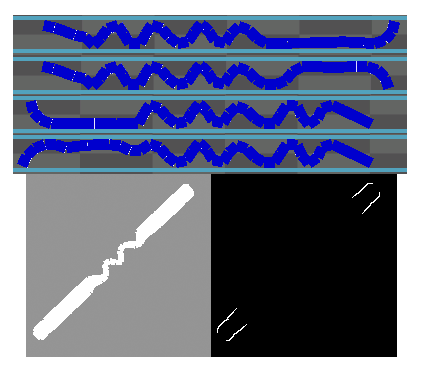
\includegraphics[scale=0.7]{PokeBehavior.png}
  \end{center}
  \caption{TODO: Remove the obstacle map.  Free space map from PokeWalls behavior.}
	\label{pokeBehavior}
\end{figure}

The map is achieved by rigidly anchoring to the environment and maintaining a set of stable reference poses.  One side of the snake's body is used to sweep the free space, making multiple snapshots of the robot's posture over time and plotting them into a map.  We discuss each aspect of our approach and show the results for a varienty of environmental configurations.

The key point here is that sensing cannot be accomplished without action.  Action by itself runs the risk of disturbing the environment or causing errors in the reference pose.  Though sensing cannot be accomplished without action, action runs the risk of modifying the result.  Special care must be taken that the risk of modifying the environment is minimized.  Here, we include the robot's body in our definition of the environment so that anchor slippage is a form of environment modification.

\section{Behavior}

In order to capture as much information about the environment as we can, we need to sweep the robot's body around as much as possible while trying to cover as much space as possible without losing our reference pose to the global frame.  Therefore, we have devised a behavior assemblage that separates responsibility for anchoring on one half of the snake and for probing the environment with the other.  This assemblage is shown in Figure \ref{pokewalls1}.  The resulting behavior is shown in Figure \ref{pokeBehavior}.

The resultant behavior sweeps the front end of the snake back and forth, impacting both sides of the pipe.  The front is gradually extended to increase the probe reach down the pipe.  Once the extension has reached the maximum, the behavior is terminated after returning the snake back to its original fully anchored Rest-State posture.

At regular intervals during the sweeping behavior at the end of each Transition termination, the posture is recorded for later processing.  The end result is an ordered list of posture vectors representing each snapshot of the robot during the behavior.  These postures are then processed into a map.

We describe each behavior in the assemblage.


\begin{figure}
\begin{center}
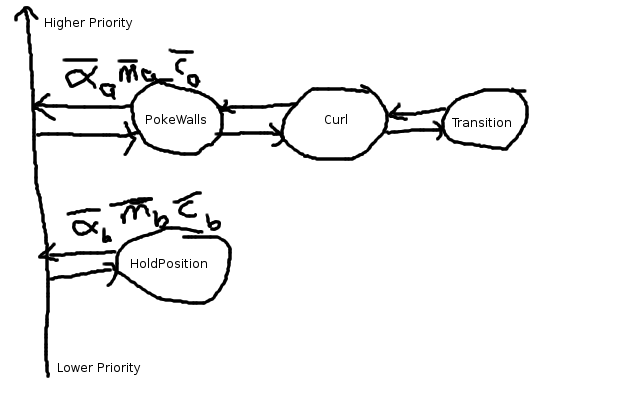
\includegraphics[scale=0.5]{4_pokewalls_1.png}
\end{center}
\caption{PokeWalls behavior assembly.}
\label{pokewalls1}
\end{figure}

%GRAPHIC
%Merge(
%PokeWalls <- Curl <- Transition
%HoldPosition
%)



\textbf{Curl:} The sweeping behavior is performed by setting a series of consecutive joints all to a 30 degree angle, resulting in a curling motion.  In a confined environment, the result of the commanded joints usually results in the snake impacting the walls of the environment.  By steadily increasing the number of joints to perform this sweeping motion, the reach of the snake is gradually increased and more space is sweeped out.

The Curl sub-behavior is responsible for commanding these joint angles given the specified joint range by the parent.  It is also responsible for executing a simple contact detection heuristic in the course of the curling behavior.  We describe both here.  

Given the top joint $j_t$ specified by the parent, the Curl behavior gives commands to the joints $(j_0 ... j_t)$, setting $\alpha_i = 0$.  All $\alpha$ are set to the following sequence of angles: $(0, 25, 30, 0, -25, -30, 0)$.  Between each movement command we use the Transition sub-behavior to manage the motion as a linear interpolation between postures.  We also wait for the tip of the snake's position to become stable for executing another movement transition.  At the end of the movement sequence and once the tip has become stable, the Curl behavior then terminates and waits to be reset by the parent. 

For the contact detection heuristic, once the joints have been set to $\alpha = 25$, the tip of the snake's position $p_a$ is computed kinematically.  The joints are then set to $\alpha = 30$ and the tip's position $p_b$ is again computed kinematically.  The Cartesian distance between $p_a$ and $p_b$ is computed.  If the value is negligible, we assume that the tip of the snake has made contact with the walls.  Otherwise, we do not assume contact has bee made.  The repeat this for the negative angle commands on the other side of the pipe.  

The way the sweeping behavior is performed is by setting the commanded position of all the joints from the tip of the snake down to a top joint simultaneously from 0 to 30 degrees.  This results in a "curling" behavior which gives the subbehavior its name.  The joints are set at angles of 0, 25, 30, 0, -25, -30, 0.


%- Curl sub-behavior
%- set all joints to -30, -25, 0, 25, 30
%- from top joint to tip
%- skip back to 0 from terminator
%- check difference between |30| and |25| to see if contact is made

\textbf{PokeWalls:} The PokeWalls behavior is responsible for specifying the range of joints that perform the Curl operation, instantiating and configuring the Curl behavior.  The PokeWalls behavior is configured with the sweeping direction on the snake, starts the Curl behavior with the joint range specified by $j_t = 6$.  It then passes through the outputs of the Curl behavior.

At the termination of the Curl behavior, PokeWalls increments $j_t$ by 2 and restarts the Curl behavior with the new parameters.  If $j_t = 10$, we then begin decrementing $j_t$ by 2 until we go back to $j_t = 6$.  Once the Curl has been executed for the second for $j_t = 6$, we terminate the PokeWalls behavior.

The PokeWalls behavior is also responsible for setting the maximum torque for each of the curling joints to be compliant.  This ensures that the posture of the snake complies to the environment and gives us as much information as possible about the structure of the free space.  If we do not have compliant joints, the curling behavior can result in disruption of the anchors and loss of our reference poses.

%is to specify which joints participate in the sweeping behavior and spawns the Curl sub-behavior.
%- receives direction
%- sets the top joint from 6 to 10 on Curl
%- walks it through Curl steps, resets and does topJoint
%- sets compliant torque from 0 to topJoint
%- sets top joint from 6 to 10 to 6 and then terminates

\textbf{Transition:}   This is the same behavior as described in Chapter 2.  It takes an initial and final posture and outputs a series of postures that provides a smooth transition between the two using interpolation.  Its parent behavior is Curl which instantiates it and resets it whenever it needs to perform a new move.

\textbf{HoldPosition:} This is the same behavior as described in Chapter 2.  It is initialized with the complete posture of the snake at the beginning of the behavior.  This posture is usually the result of the Rest-State stage of the Adaptive Step locomotion process.  It continually outputs the anchored posture.  Its output is subsumed by the output from the PokeWalls behavior in a precedence merge.  It is 2nd in the behavior ordering as shown in Figure \ref{pokewalls1}. 




\section{Proprioceptive Sensor Data}

Now that we've specified the actions we perform to sense the environment by way of the PokeWalls and Curl behavior, we now need to show how we capture sensor data and process it for consumption for our later mapping algorithms.

\subsection{Data Capture}

Once the posture of the snake has stabilized and the anchor points give us good reference poses to the global frame, our objective is take the posture vector, $\bar{\phi_t}$ at time $t$, and convert it to a 2D spatial representation of free space, $M_p$ at the current pose $p$.  We separate the tasks of spatial representation and positioning the data in the global frame.  To do this, we create a local map centered on the robot's body on which the spatial data is plotted while the robot remains in one position.

The local map is an occupancy grid representation where each cell of the grid has two states:  \emph{unknown} or \emph{free}.  If the body of the robot is present on a cell, this cell is marked \emph{free}.  Otherwise, it is \emph{unknown}.  It is unknown instead of \emph{occupied} because our approach does not have any means to specifically observe obstacles beyond contact detection heuristics.  The heuristics are not accurate enough to plot their positions into the occupancy grid, so we leave the cells unknown for now.

The size of a cell is chosen for the desired accuracy we require.  Smaller cell sizes require more computational time, but larger cell sizes will result in blocky maps.  We choose our cell dimensions $s_p \times s_p$ to be
%pixelSize
$s_p = \frac{l}{3} = 0.05$, or one third the length of a snake segment.

Given that we now have our cell dimensions, we can compute the dimensions of our local map to be 
%mapSize
%$s_M = l * N+ 2 + 2$,
$s_M = l * N$ + 4,
where $l$ is the segment length and $N$ is the number of segments.  $s_M$ is the maximum length from the origin at the center of our local coordinate system.  We want the dimensions to be larger than the worse case scenario of the snake's posture.  We also include an extra padding of $4$ to ensure that the snake never reaches the boundary of the grid.

The number of cells or pixels in our local map will be $n_p \times n_p$ where
%numPixel
$n_p = \bigg\lceil \frac{2 s_M}{s_p} + 1 \bigg\rceil$.  This equation ensures that $n_p$ is an odd integer.  The $+1$ factor adds an extra cell whose center will act as the origin of our local coordinate system.


Now that we have the dimensions of the grid space and its relation to Cartesian space, we need to know how to convert points from one space to the other.  To convert a grid index $(i_x,i_y)$ to Cartesian space point $(p_x,p_y)$ centered within the cell, we compute the following:
%$p_x = (i_x - n_p/2 - 1)*(s_p/2) + s_p/2$
%p_y = (i_y - n_p/2 - 1)*(s_p/2) + s_p/2$
\begin{eqnarray}
\label{eqn:g_to_p}
%p_x = \bigg(i_x - \frac{n_p}{2} - 1\bigg)\frac{s_p}{2} + \frac{s_p}{2} \\
%p_y = \bigg(i_y - \frac{n_p}{2} - 1\bigg)\frac{s_p}{2} + \frac{s_p}{2} 
p_x = \bigg(i_x - \bigg\lfloor\frac{n_p}{2}\bigg\rfloor \bigg)\frac{s_p}{2} \\
p_y = \bigg(i_y - \bigg\lfloor\frac{n_p}{2}\bigg\rfloor \bigg)\frac{s_p}{2}
\end{eqnarray}


Conversely, to find the index of a cell $(i_x,i_y)$ that contains a Cartesian point $(p_x,p_y)$, we compute the following:
%divPix
%$divPix = \lfloor \frac{\frac{2 s_M}{s_p}}{s_M} \rfloor$
%$i_x = \lfloor point[0]*2/s_p \rfloor + n_p/2 + 1$
%$i_y = \lfloor point[1]*2/s_p \rfloor + n_p/2 + 1$
\begin{eqnarray}
i_x = \bigg\lfloor \frac{p_x}{s_p} \bigg\rceil + \bigg\lceil\frac{n_p}{2}\bigg\rceil \\
i_y = \bigg\lfloor \frac{p_y}{s_p} \bigg\rceil + \bigg\lceil\frac{n_p}{2}\bigg\rceil
\end{eqnarray}


Now that we have the tools for mapping positions in physical space to our grid space occupancy map, we need data to plot into the map.  Using kinematics, we compute the geometry of the posture of the snake.  We can represent this by a 4-sided rectangle for each segment of the snake.  We set the origin of our coordinate system on segment 19 and joint 19 which is the midway point for $N = 40$.  We define this to be:
\begin{equation}
O_t = (x_{19}, y_{19}, \theta_{19}) = (0, 0, 0)
\end{equation}
where $O_t$ is the pose of $P_{19}$ in the local frame at time $t$.  This may change which is explained in section \ref{sec:ref_stable}.

To compute the segment 19 rectangle, starting from the origin for $k = 19$, $x_k = 0$, $y_k = 0$, and $\theta_k = 0$, we compute the following:

%From 19, towards N
\begin{equation}
\label{equ:rect1}
\begin{array}{l}
\displaystyle x_{k+1} = x_k + l \cos(\theta_k) \\
\displaystyle y_{k+1} = y_k + l \sin(\theta_k) \\
\displaystyle \theta_{k+1} = \theta_k - \phi_{k+1} \\
\displaystyle p_1 = \bigg( x_{k+1} - \frac{w\sin(\theta_k)}{2} , y_{k+1} + \frac{w\cos(\theta_k)}{2}\bigg) \\
\displaystyle p_2 = \bigg( x_{k+1} + \frac{w\sin(\theta_k)}{2}, y_{k+1} - \frac{w\cos(\theta_k)}{2} \bigg) \\
\displaystyle p_3 = \bigg( x_{k+1} - l\cos(\theta_k) + \frac{w\sin(\theta_k)}{2}, y_{k+1} - l\sin(\theta_k) - \frac{w\cos(\theta_k)}{2} \bigg) \\
\displaystyle p_4 = \bigg( x_{k+1} - l\cos(\theta_k) - \frac{w\sin(\theta_k)}{2}, y_{k+1} - l\sin(\theta_k) + \frac{w\cos(\theta_k)}{2} \bigg) \\
\displaystyle R_k = (p_4,p_3,p_2,p_1)
\end{array}
\end{equation}

The result is the rectangle polygon $R_k$, which represents the rectangle of the segment $19$.  The next reference pose $(x_{k+1},y_{k+1},\theta_{k+1})$ is also computed.  Here $k+1=20$.  To compute the k\textsuperscript{th} rectangle for $k \geq 19$, we need only compute this iteratively until we reach the desired segment.

To perform this backwards, to find segment $18$, where $k+1=19$ and $(x_{k+1}, y_{k+1}, \theta_{k+1}) = O_t$, we compute the following:

\begin{equation}
\label{equ:rect2}
\begin{array}{l}
\displaystyle \theta_k = \theta_{k+1} + \phi_k \\
\displaystyle x_k = x_{k+1} - l \cos(\theta_k) \\ 
\displaystyle y_k = y_{k+1} - l \sin(\theta_k) \\
\displaystyle p_1 = \bigg( x_{k+1} - \frac{w\sin(\theta_k)}{2} , y_{k+1} + \frac{w\cos(\theta_k)}{2}\bigg) \\
\displaystyle p_2 = \bigg( x_{k+1} + \frac{w\sin(\theta_k)}{2}, y_{k+1} - \frac{w\cos(\theta_k)}{2} \bigg) \\
\displaystyle p_3 = \bigg( x_{k+1} - l\cos(\theta_k) + \frac{w\sin(\theta_k)}{2}, y_{k+1} - l\sin(\theta_k) - \frac{w\cos(\theta_k)}{2} \bigg) \\
\displaystyle p_4 = \bigg( x_{k+1} - l\cos(\theta_k) - \frac{w\sin(\theta_k)}{2}, y_{k+1} - l\sin(\theta_k) + \frac{w\cos(\theta_k)}{2} \bigg) \\ 
\displaystyle R_k = (p_4,p_3,p_2,p_1)
\end{array}
\end{equation}

The result is the same polygon as well as the new reference pose for segment $18$.  To compute the k\textsuperscript{th} segment rectangle for $k < 19$, we need only use this equation iteratively.  Computation of all $N$ rectangles results in the set of rectangles $\bar{R_t}$ for the current posture.

Now that we have a set of rectangles which represent the geometry of the robot in its current posture, we want to plot its occupied space into the local occupancy map.  To do this, we need to convert polygons in Cartesian space into sets of grid points.  To do this, we use a point-in-polygon test algorithm for each of the pixels in the map.

The simplest approach is as follows.  For each pixel, convert it to Cartesian space, test if it's contained in any of the polygons, and if it is, set the pixel to \emph{free}.  Otherwise, let the pixel remain in its current state.  The pseudocode for the point-in-polygon test for convex polygons derived from \cite{orourke98} is seen in Algorithm \ref{alg:pip_test}.

\begin{algorithm}
\caption{Point-in-Polygon Test}          % give the algorithm a caption
\label{alg:pip_test}
\begin{algorithmic}

\State $R \Leftarrow $ rectangle
\State $P \Leftarrow $ point

\For{$i = 0 \to 4$}
\State $A_x \Leftarrow R[i \bmod 4][0] $
\State $A_y \Leftarrow R[i \bmod 4][1] $
\State $B_x \Leftarrow R[(i+1) \bmod 4][0] $
\State $B_y \Leftarrow R[(i+1) \bmod 4][1] $
\State $C_x \Leftarrow P[0] $
\State $C_y \Leftarrow P[1] $

\If{$!((Bx - Ax) * (Cy - Ay) - (Cx - Ax)*(By - Ay) \geq 0)$}
\State return False
\EndIf
\EndFor
\State return True

\end{algorithmic}
\end{algorithm}

\begin{figure}
  \begin{center}
    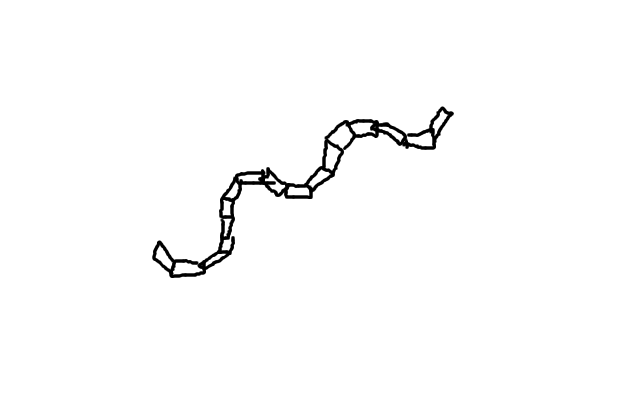
\includegraphics[scale=0.7]{4_snapshot_1.png}
  \end{center}
  \caption{Snapshot of $\bar{\phi_t}$ in local coordinates.}
	\label{snapshot}
\end{figure}


A single snapshot of the snake posture plotted into the local map is shown in Figure \ref{snapshot}.  The posture $\bar{\phi_t}$ is captured, the rectangles $\bar{R_t}$ representing the body segments are computed from kinematics, each pixel $(i_x,i_y)$ of the map $M_p$ is converted to Cartesian space point $(p_x,p_y)$ and checked by the point-in-polygon algorithm if it is in a rectangle $R_k$.  If it is, $M_p(i_x,i_y)$'s value is set to \emph{free}.  This is repeated for each point in each rectangle for a posture snapshot at time $t$.

\begin{figure}
  \begin{center}
    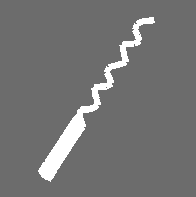
\includegraphics[scale=1.0]{localOccMapSingle0.png}
  \end{center}
  \caption{Single forward sweep. }
	\label{single_sweep}
\end{figure}

\begin{figure}
  \begin{center}
    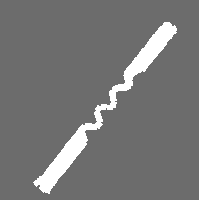
\includegraphics[scale=1.0]{localOccDouble.png}
  \end{center}
  \caption{Forward and backward sweep.}
	\label{double_sweep}
\end{figure}



While running the PokeWalls behavior, we periodically take snapshots at the conclusion of each Transition step and plot them into the map.  A complete sweep with the PokeWalls behavior is shown in Figure \ref{single_sweep}.   Furthermore, if we also perform a sweep with the other side of the snake, we can get a map like Figure \ref{double_sweep}.

Notice in Figure \ref{double_sweep} that there is a gap in the free space data in the center of the body.  These segments at the center remain immobilized throughout the sweeping process and never give extra information.  This gap in the center is our "blind spot" for this configuration.  It is necessary that the center remain immobilized to ensure anchors do not slip so that we maintain correct reference poses to the global frame.

We have no guarantee that there are obstacles at the boundaries of our free space map.  We also have no quick way to determine if the boundary of our map is an obstacle or a frontier.  While the boundaries at the front and back are usually assumed to lead to more free space, anywhere along the sides could be a missed side passage that the snake failed to discover due to it being too small or being in our blind spot.  To combat this situation, we either must perform laborious and time-consuming contact probing of every surface, or use quick-and-dirty contact detection heuristics to guide our mapping process.

\subsection{Data Processing}

Once we have the raw sensor data successfully plotted into a local occupancy map, we must convert this data into a form that is useful for our mapping algorithms.  Here, we present three different forms of data processing that we use in our approach.

\subsubsection{Convex Hull}

One way we process our free space data is by taking its convex hull.  In theory, this would create some smooth boundaries and can plausibly represent the true local space under some certain conditions.   The definition of the convex hull is, given a set of points $P$, find the convex polygon $H$ with minimum area that contains all of $P$.

To create our set of points $P$, for each pixel $(i_x,i_y)$ of the occupancy map $M_p$ whose state is \emph{free}, convert the pixel to Cartesian space point $(p_x,p_y)$ using Equation \ref{eqn:g_to_p} and add to $P$.  Using any convex hull algorithm, produce the resultant polygon in Cartesian space.   For our work, we use the convex hull algorithm available in CGAL \cite{cgal:hs-chep2-12b}.

\begin{figure}
  \begin{center}
    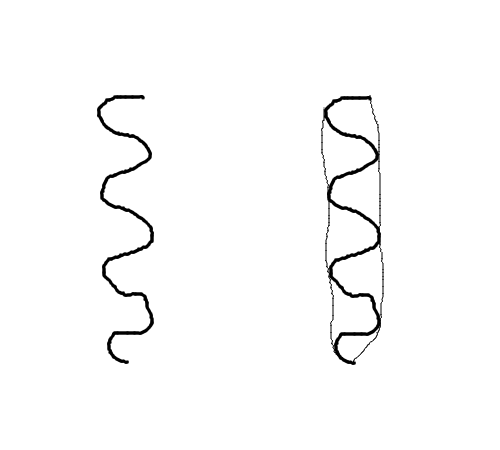
\includegraphics[scale=0.9]{4_convex_freespace1.png}
  \end{center}
  \caption{Free space data before and after convex hull.}
	\label{convex_free1}
\end{figure}

\begin{figure}
  \begin{center}
    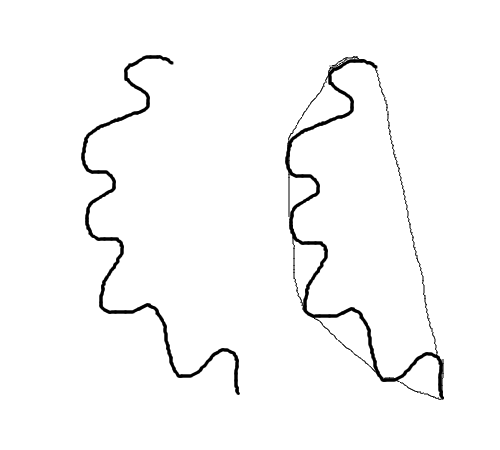
\includegraphics[scale=0.9]{4_convex_freespace2.png}
  \end{center}
  \caption{Free space data of curved posture before and after convex hull.}
	\label{convex_free2}
\end{figure}

An example of the convex hull operation on our free space data set appears in Figure \ref{convex_free1}.  We can see for the case that the snake is in a straight pipe, the convex hull creates a natural representation of the local pipe environment, filling in the blanks of our blind spot.  However, if the pipe is curved as in Figure \ref{convex_free2}, the convex property of the polygon necessarily erases any concave properties of the environment.  This also removes any sharp features of the environment such as corners.  Therefore, any use we may have for the convex hull will be in limited situations.


%A common algorithm from computational geometry that finds a minimum convex polygon that fits all the points.  The points in our case are the grids that are marked with free space.   Convert theses pixesl to points at their centers, and we have input for a convex polygon.  The results look like Figure 0.  Cite \cite{cgal:hs-chep2-12b}

%This has the capability of smoothing over the gaps from the blind spots.  Has shortcomings.  Loses corners.

%Has some uses, but for curved pipes, we lose critical information about the true pipe dimensions and their curved topology.  Does not represent nonconvex features.

\subsubsection{Alpha Shape}

An alternative to the convex hull is the alpha shape \cite{Edelsbrunner:1983p772}.  Like the convex hull, it creates a polygon or polygons that contain all the points.  Unlike the convex hull, it can construct a containing polygon with concave or even hole features.  

\begin{figure}
  \begin{center}
    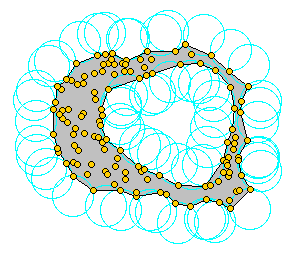
\includegraphics[scale=0.7]{alphashape.png}
  \end{center}
  \caption{Alpha Shape example from \cite{cgal:d-as2-12b}}
	\label{alpha_cgal}
\end{figure}

To construct the alpha shape, first we choose a radius $r$ for a circle $C$.  Next, if a pair of points $p_i$ and $p_j$ can be put on the boundary of $C$ where no other point is on or contained by $C$, we add an edge between $p_i$ and $p_j$.  The result is seen in Figure \ref{alpha_cgal}

\begin{figure}
  \begin{center}
    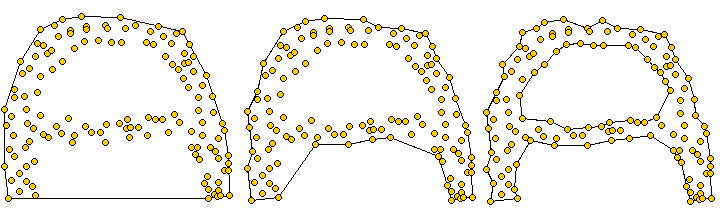
\includegraphics[scale=0.6]{4_alpha_radius.png}
    %\includegraphics[scale=0.7]{alpha_example2.gif}
  \end{center}
  \caption{Alpha Shape changing radius from \cite{cgal:d-as2-12b}}
	\label{alpha_cgal2}
\end{figure}

By changing the radius size, we can tune how much smoothing we want to occur in the resultant polygon, seen in Figure \ref{alpha_cgal2}.  If we set the radius to $r = \infty$, the alpha shape reduces to the convex hull.  Therefore, this is a kind of "generalized convex hull" algorithm.

\begin{figure}
  \begin{center}
    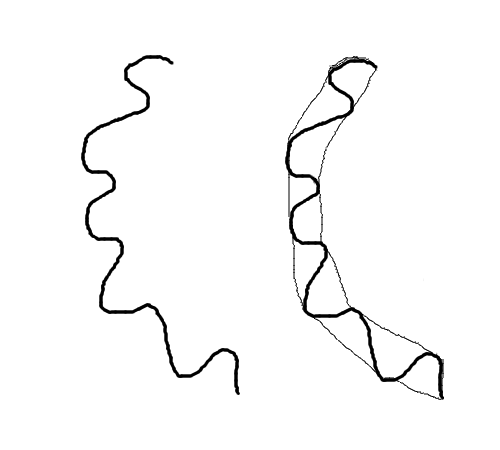
\includegraphics[scale=0.9]{4_alpha_freespace2.png}
  \end{center}
  \caption{Alpha hull of free space data.}
	\label{alpha_free2}
\end{figure}

The benefit to this approach is that we can now capture the concave features of some of our local maps where the convex hull failed.  Where Figure \ref{convex_free2} shows the convex hull, Figure \ref{alpha_free2} shows its corresponding alpha shape.  In both cases, the blind spot it smoothed over and filled in.  This approach still suffers from the loss of sharp salient corner features, but the gross topology of the local environment has been captured.

For clarity, we refer to the alpha shape of our local free space as the \emph{alpha hull} from here on out.


\subsubsection{Medial Axis}

Although polygons that represent the sweeped free space are useful, we need something that is more compact that also filters out the smoothing effects of blind spots and sharp features.  That is, we want an approach where the negative effects of missing data, erroneous data, and loss of salient features are minimized.

For this purpose, we compute the medial axis, also sometimes known as thinning or skeletonization [cite].  This concept takes a shape and reduces it to a path or series of edges that follow the "spine" of a shape.  Approaches range from a strict computational geometry approach such as the Voronoi diagram to image processing approaches of image thinning and skeletonization that erode a pixelized shape until the skeleton is all that remains [cite].

%Skeletonization of a binary image.
%Black values (0) mean object and white values (1 = 255) background.
%Source: Parker, J.R. Algorithms for image processing and computer vision.
%				New York, NY: John Wiley & Sons, 1997. 417p. pp. 203-218.
%
%Program adapted to C/OpenCV by Jose Iguelmar Miranda.
%March, 2010.
%I have also a Java version of this program.

\begin{figure}
  \begin{center}
    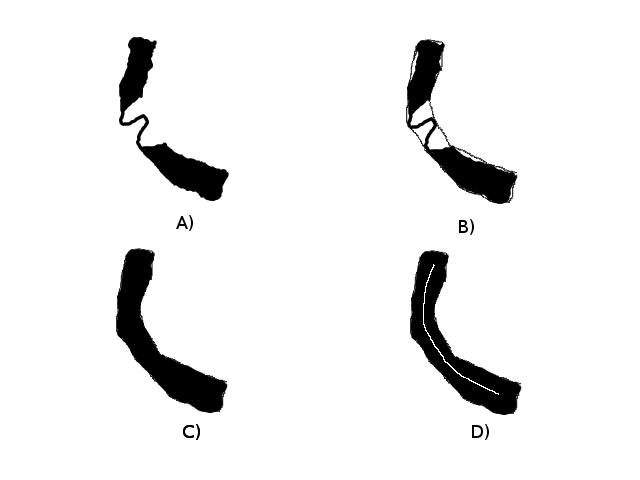
\includegraphics[scale=0.9]{4_medial_process.png}
  \end{center}
  \caption{Process of generating medial axis.}
	\label{medial1}
\end{figure}

\begin{figure}
  \begin{center}
    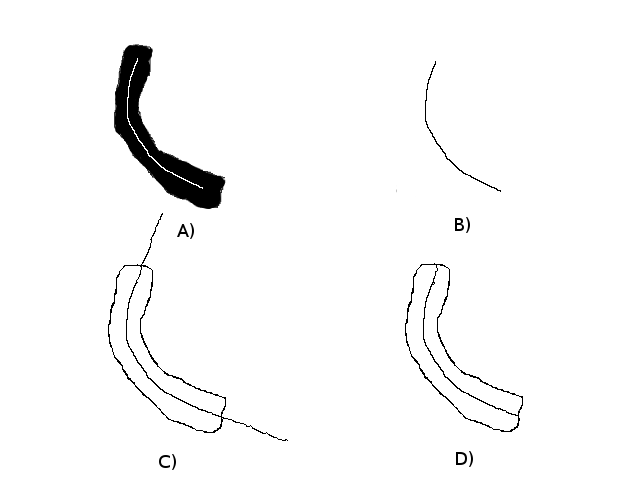
\includegraphics[scale=0.9]{4_medial_process2.png}
  \end{center}
  \caption{Process of generating medial axis.}
	\label{medial2}
\end{figure}

We are interested in extracting the medial axis of the alpha hull generated from our free space map.  Since the alpha hull smooths the boundaries of the free space map, generating a medial axis will give us a topological representation of the free space that is resistant to boundary features.  Given the free space map in Figure \ref{medial1}a, and its corresponding alpha hull in Figure \ref{medial1}b, the alpha hull's conversion back to an image in Figure \ref{medial1}c, and its resultant medial axis shown in Figure \ref{medial1}d.  We use the skeletonization algorithm from [ParkerJR] \footnote{C/OpenCV code written by Jose Iguelmar Miranda, 2010}.

We can see that the medial axis roughly corresponds to the topological representation of the pipe environment.  However, it is crooked, pixelated, and does not extend the full length of the data set.  We further treat this data to give a more useful representatation.

Starting with the result from Figure \ref{medial1}d shown in Figure \ref{medial2}a, we create a minimum spanning tree (MST) graph where each node is a pixel from the medial axis and an edge is added between two nodes if their corresponding pixels are neighbors, shown in Figure \ref{medial2}b.

This MST has many leafs due to the artifacts of pixelation.  We can simply prune the whole tree by sorting all nodes by degree, and removing the nodes with 1 degree and their corresponding edges.  In most cases, this will leave us with a single ordered path of nodes with no branches.  In some cases, we will have a branch if the original free space map shows evidence of a junction.

In the case of a single path, our next step is to extend this path to full extent of the original shape.  We begin by fitting a B-Spline curve to the ordered path.  With an appropriate smoothing parameter, the spline curve will follow the path of the ordered points but will ignore the jagged edges from pixelation.  We then uniformly sample points along this curve to convert it back to an ordered set of points.  We extend this path in the front and back by extrapolating more points along the direction specified by the curve tip, as in Figure \ref{medial2}c.  Multiple tangent vectors are sampled along the tip neighborhood and their direction is averaged to get a direction that is immune to spline curving artifacts at the terminals.  Finally, the series of points is cut off once the extrapolated points cross the alpha hull boundary, shown in Figure \ref{medial2}d.

In the case that we have a branch, we perform this series of operations for the path between each combination of pairs of terminals.  For each medial axis of a free space map, there are $n = 2 + B$ end points where $B$ is the number of branches.  The number of unique paths of a medial axis is found by ${n \choose 2}$ since we are using the MST and there is a unique path between each pair of points.

The final form is a compact representation of the topology of the local free space that removes the noise and uncertainty of the boundary and allows us to only represent the area we can move through.  This has a number of uses for our map-making that we describe in the next chapter.  

% environment -> free space map -> alpha hull -> image of alpha hull interior -> medial axis -> graph -> MST -> Spline -> sampled points -> extrapolation -> cutoff at boundary -> overlap of environment 

\section{Failures}

Since the possibility of error occuring in our free space maps is very real and has the consequences of making the data near-useless, we want to do all we can to prevent and mitigate any failure conditions.  As the primary source of error is anchor slip, we do all we can to focus on this issue while probing the environment.  We use a number of techniques for both prevention and detection of error.  We describe all of our approaches below.

\subsection{Error Prevention}

We have 6 strategies for preventing anchor slip during the course of probing the environment.  These are the following:

\begin{enumerate} \itemsep 1pt \parskip 0pt \parsep 0pt
  \item Prescriptive Stability
  \item Local Stability
  \item Smooth Motion
  \item Averaging Reference Poses
  \item Separation of Sweep Maps
\end{enumerate}

The first three we have discussed earlier, with prescriptive stability and local stability in section \ref{sec:anchors} and smooth motion in section \ref{sec:smooth}.  We use prescriptive and local stability to determine which reference poses are available to be activated.  Whereas, smooth motion through the use of linearly interpolated steps by using the Transition behavior reduces the chance that our anchors will slip. 

The prescriptive stability selection of the PokeWalls behavior requires the robot to only use the anchored portion of the snake body for reference poses.  In particular, it is very conservative, where only the segments at the very back and mechanically isolated from any of the sweeping motions in the front will be used for reference.  This reduces the chance that any perturbations from the probing motions will have an effect on any of the active reference poses that we are using.

\subsubsection{Averaging Reference Poses}

For our fourth strategy, when actually using the reference poses to compute the position of the snake in our local free space map, we want to use as many of the reference poses as possible while filtering out any errors that would occur from possible pathological cases.   If just one reference pose is erroneous and we use that reference pose to compute position of the snake in free space,  it will severely damage our results.  We want to mitigate the possibility of negative effects by taking the average of a set of reference poses when computing a snake's position.

For instance, if we wanted to compute the origin of our local free space map in global space, we would compute the kinematic position of joint 19 with respect to some active reference pose $P_k$ on joint and segment $k$.  Using equation \ref{kinem1} or \ref{kinem2}, we compute the position of $P^{k}_{19}$.  For every $P_k$ we use, we compute a new $P^{k}_{19}$ that is possibly different.  We then take the average of all of the computed $P^{k}_{19}$ poses and take that as our best guess for $P_{19}$. 

\begin{figure}
  \begin{center}
    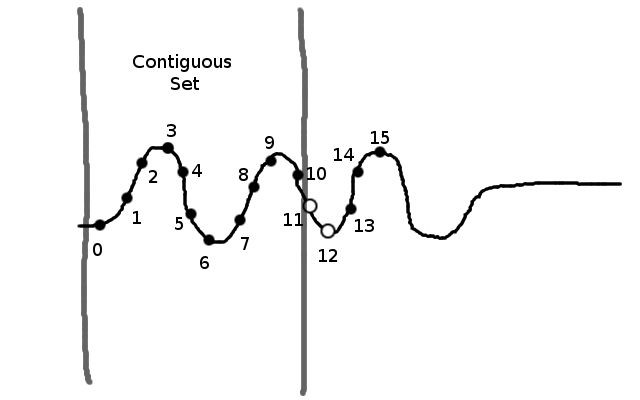
\includegraphics[scale=0.6]{4_ref_averaging.png}
  \end{center}
  \caption{Largest set of contiguous reference poses.}
	\label{ref_average}
\end{figure}

How do we select the set of active reference poses from which to compute our estimated snake pose?  Of all available active reference poses, our approach is to use the largest set of contiguous poses to compute the average target pose $P_{19}$.   Our assumption is that if we have a series of reference poses from 0 to 15, and 11 and 12 are deactivated, it is highly possible that 13, 14, and 15 are invalid because whatever caused 11 and 12 to be activated will likely have an effect on its neighbors.  The larger section from 0 to 9 has less likelihood of being corrupted since more of our sensors indicate stability.  Furthermore, if one or two of these reference poses are corrupted, having a larger set reduces the weight of an erroneous value.  This example is shown in Figure \ref{ref_average}.

\subsubsection{Separation of Sweep Maps}

Our fifth and final strategy for preventing errors in our sensor maps is to divide the forward sweep phase and backward sweep phase into separate maps.  From our experiments, we determined that a consistent source of error occurs when switching the anchoring responsibility from the back half of the snake to the front half.  The series of events of retracting the front half of the snake to anchors and extending the back half for sweeping tends to cause some discontinuity between the consensus of the back reference poses and the front reference poses.  This will show with a very distinct break in the combined free space map.

\begin{figure}
  \begin{center}
    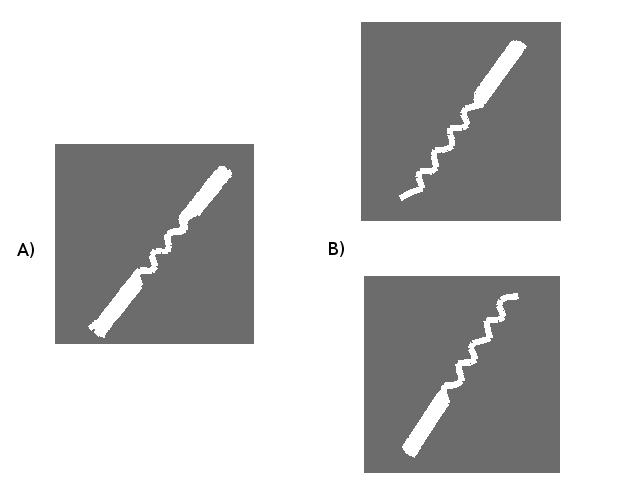
\includegraphics[scale=0.6]{4_sweepmap_1.png}
  \end{center}
  \caption{Separation of Sweep Maps.}
	\label{ref_sweep_sep}
\end{figure}

To avoid this problem, we instead create two free space maps: one for the front sweep and one for the back sweep.  What was previously shown in Figure \ref{ref_sweep_sep}a will now become the pair of maps shown in Figure b.  Not only does this avoid corrupting the free space data in the map, but it allows us to treat the relationship between the two maps as a separate problem for which there are multiple solutions.  Our previous sensor processing algorithms work just as well because the alpha shape of the half-sweep free space map will result in an alpha hull from which an equivalent medial axis can be extracted.  

We discuss our approach to managing the relationship between the two half-sweep local maps in the next chapter.

%The fourth strategy is in regard to how to use the reference poses to compute the pose of a robot segment in space.  Instead of selecting one reference pose to use and hoping that it is 100 percent correct, we take a set of reference poses and average the computed position of a target segment.  How we select the set of references to use is by looking for the largest contiguous set.  That is, reference poses that are active and are all neighbors, we select the largest set.  If for instance, a set of 15 reference poses are used in time $t$ and later reference pose 10 becomes deactived, for time $t+1$, we assume that the poses $0-9$ are still immobile and not $11-15$.  Our heuristic assumes that it is much easier to move less segments than more.  

%-- averaged position from the back anchor reference poses

%-- only use backy-back reference poses to minimize possibility of bad reference poses being used.   Prescriptive stability is very conservative.

% Separation of forward sweep and backward sweep local maps.  Do not merge them but keep them separate and correctable.
% Error comes from the switch in posture from back-anchor/forward sweep to front-anchor/backward sweep


\subsection{Error Mitigation}

In the case that error is introduced into our local free space map, we are interested in mitigating its negative effects.   We have developed two approaches for handling error when it occurs during sensing.

Since we start our mapping process by determining the global pose of the local origin $P_{19}$, error occurs when $P_{19}$ is no longer in its proper place.  Either it moves by translation or more commonly and critically, it experiences rotational error.  

\subsubsection{Reference Stabilization}
\label{sec:ref_stable}

\begin{figure}
  \begin{center}
    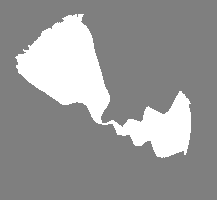
\includegraphics[scale=1.0]{localMapError.png}
  \end{center}
  \caption{Local map rotational error.}
	\label{ref_rot_error}
\end{figure}

A sudden rotation of $P_{19}$ may occur, caused by any of the reasons detailed in Section \ref{sec:anchors}.  The consequences of rotational error is that the entire body of the snake will rotate around the origin within the local map.  This will result in a map feature shown in Figure \ref{ref_rot_error}.

We proactively combat this possibility by running a reference stabilization algorithm that continually corrects the local origin $O_t$ for $P_{19}$ in the local map at time $t$.  For $t=0$, the origin is $(0,0,0)$ for inputing into the equations \ref{equ:rect1} and \ref{equ:rect2}.  However, for each time step, we wish to calculate an $O_t$ that is the most "stable" in case $P_{19}$ becomes destabilized.

To do this, we remark that during the probing phase, the back anchored section of the snake as a whole will remainly roughly in the same tight space even if its joints and ssegments should wobble and slip.  Short a large amount of translational slipping down the pipe, taken as a whole, the body should remain in the same place.  Therefore, in the local free space map, the back anchored portion should of the snapshot time $t$ should also remain in the same neighborhood of the back anchor snapshot at time $t-1$.  

\begin{figure}
  \begin{center}
    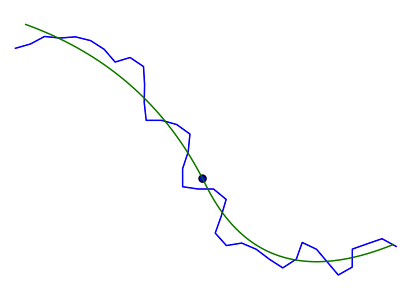
\includegraphics[scale=1.0]{plotGPAC0059.png}
  \end{center}
  \caption{Gross Posture Approximation Curve of sample posture.}
	\label{ref_gpac}
\end{figure}

We enforce this observation by fitting B-spline curve $\beta_t$ and $\beta_{t+1}$ along the points that make up the reference poses of the back anchor segments for both the current and previous snapshots.  The B-spline curves are calibrated to smooth out the sinusoidal anchoring posture of the snake body and instead reflect the gross posture of the body in the confined environment as shown in Figure \ref{ref_gpac}.   We then find a $(\delta x, \delta y, \delta \theta)$ for $\beta_{t+1}$ such that the two curves are aligned and then we update $O_{t+1}$ to reflect this.

This approach prevents sudden rotational errors from occurring and corrects the snake's estimated pose in the local map while we are capturing sensor data by generating a new $O_{t+1}$ that is consistent with past data.  So even if the snake's body is wobbling or slipping, we will likely produce consistent sensor data.
 

%Our goal is to detect when this first occurs and compensate to keep the map consistent.  We accomplish this by determining if the new posture snapshot suddenly jumps out of the local free space area we have already mapped.  The time between snapshots is very short and the snake probe is moving slowly enough that this is a reasonable assumption.

%We accomplish this by doing the following.   At every timestep $t$, we have previously computed the alpha hull $H_{t-1}$ for the current free space map.   For the current posture $\bar{\phi_t}$, and for its position in the free space map using equations \ref{equ:rect1} and \ref{equ:rect2} and starting from the origin $O_{t-1}$, determine if its position breaches the boundary of $H_{t-1}$ by distance $d_h$.

%--- we suppose that a significant rotational error has occurred.  In this case, we alter the location of the root pose from origin to an offset that keeps the posture inside the polygon boundary.  
%--- Correction is achieved by creating a spline of the back segments of the original and the current back posture.  The back splines are re-aligned and the pose of the root node is recomputed using this is a constraint.

\subsubsection{Minimum Data Reduction}

If all of our error prevention and reference stabilization strategies fail and we still produce corrupted data, we wish to detect this fact and handle it accordingly.  As we said, most error creates a rotation effect around the origin $O_t$, and produces an effect shown in Figure \ref{ref_rot_error}.  We call this sensor artifact a \emph{bowtie}.

\begin{figure}
  \begin{center}
    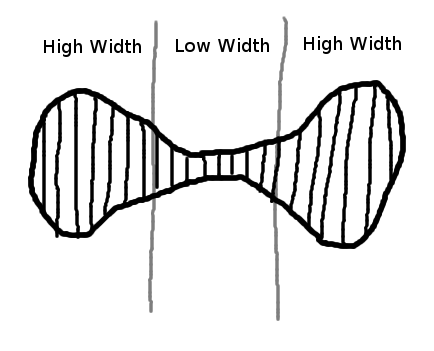
\includegraphics[scale=0.6]{4_bowtie_detect.png}
  \end{center}
  \caption{Width distribution for detecting a bowtie.}
	\label{bowtie}
\end{figure}

We develop a bowtie detector where we expect high widths on the exteriors and a tight width in the center shown in Figure \ref{bowtie}.  If we detect these conditions, then we declare this a bowtie and the proceed to the next step.  Note that this approach assumes that we will not encounter an environmental feature that approximates a bowtie.  We will address environments with bowtie features in future work.

\begin{figure}
  \begin{center}
    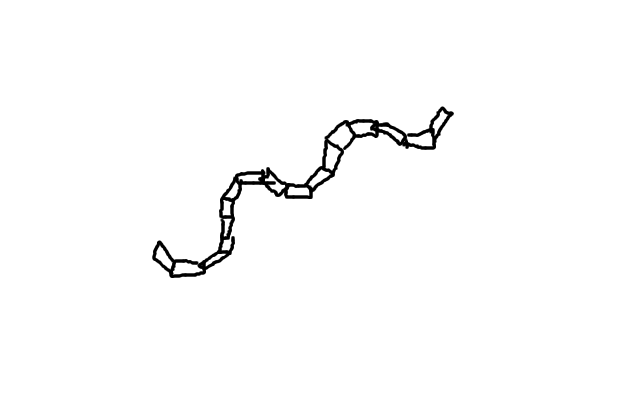
\includegraphics[scale=0.5]{4_snapshot_1.png}
  \end{center}
  \caption{FIXME: Minimum data of anchored position if bowtied: only initial posture.}
	\label{snapshot2}
\end{figure}

Once we've declared the sensor data to be bowtied, we then reduce the sensor data to minimal amount of correct information.  This would be the initial posture of the snake before it started its sweep as shown in Figure \ref{snapshot2}.  We can still treat this data with sensor processing and generate an alpha hull and a medial axis that is correct.  However, we lose data that would indicate any branches or salient wall features.  In our approach, we prefer missed data instead of bad data, so this is acceptable.

\section{Results}

